\documentclass{IOS-Book-Article}

\usepackage{mathptmx}
\usepackage[utf8]{inputenc}
\usepackage[T1]{fontenc}
\usepackage[vietnamese,english]{babel}
\usepackage{soul}\setuldepth{article}
\usepackage{float}
\usepackage{url}

\def\hb{\hbox to 11.5 cm{}}

% Math and symbols
\usepackage{amsmath,amssymb,amsfonts}
\usepackage{amsthm}
\newtheorem{definition}{Definition}

% Tables and figures
\usepackage{booktabs}
\usepackage{multirow}
\usepackage{graphicx}
\usepackage{enumitem}

% pgfplots for charts
\usepackage{pgfplots}
\pgfplotsset{compat=1.18}

\begin{document}

\pagestyle{headings}
\def\thepage{}

\begin{frontmatter}

\title{A Three-Tier Knowledge Graph RAG for Vietnamese Legal Question Answering}

\markboth{}{April 2026\hb}

% TODO: Add ORCID iDs for each author
\author[A]{\fnms{Hong Hien} \snm{Le}%
\thanks{Corresponding Author: Le Hong Hien, Faculty of Computer Science, University of Information Technology, Vietnam National University Ho Chi Minh City, Vietnam; E-mail: hienlh.16@grad.uit.edu.vn.}},
\author[A]{\fnms{Dinh Hien} \snm{Nguyen}},
\author[B]{\fnms{Quoc Hung} \snm{Ngo}}
and
\author[A]{\fnms{Viet Dung} \snm{Dang}}

\runningauthor{H.H. Le et al.}
\address[A]{Faculty of Computer Science, University of Information Technology, Vietnam National University Ho Chi Minh City, Vietnam}
\address[B]{School of Computer Science, University College Dublin, Ireland}

\begin{abstract}
Accurate legal question answering demands navigating hierarchical document structures, following cross-references, and multi-hop reasoning, capabilities that standard Retrieval-Augmented Generation (RAG) systems lack. Vietnamese legal text compounds this challenge through tonal ambiguity, domain-specific abbreviations, and rigid structural hierarchies. This paper presents a three-tier knowledge graph RAG architecture built on a formal knowledge model that integrates a domain ontology, a knowledge graph, and a document tree forest. Three retrieval tiers, LLM-guided tree traversal, dual-level semantic search with intent-aware Personalized PageRank, and Reciprocal Rank Fusion with knowledge graph expansion, operate over these representations. Evaluation on 530 expert-annotated questions across enterprise law, traffic safety law, and postgraduate education regulation shows that the proposed system retrieves at least one correct article in the top~10 results for 92.2\% of queries, outperforming the strongest baseline by 7.4\%. These results hold across all three domains without domain-specific tuning. To the best of the authors' knowledge, no prior work combines ontology-enhanced knowledge graphs with multi-tier retrieval for Vietnamese legal question answering.
\end{abstract}

\begin{keyword}
Knowledge Graph\sep Legal Question Answering\sep Retrieval Augmented Generation\sep Ontology\sep Vietnamese NLP\sep Multi-Tier Retrieval\sep Multi-Domain
\end{keyword}

\end{frontmatter}
\markboth{April 2026\hb}{April 2026\hb}

\section{Introduction}

Legal forums and social networks in Vietnam are flooded with questions on business formation, traffic penalties, and regulatory compliance. Yet answers are often fragmented, contradictory, or cite repealed provisions.

Legal documents exhibit complex hierarchical structures: a single law organizes content into parts, chapters, sections, articles, clauses, and points, where each level carries distinct legal scope. They also contain pervasive cross-references: answering ``If a member borrows money to meet charter capital and later withdraws it, what are the penalties?'' requires chaining Article~47 (member obligations) to Article~16, Clause~5 (prohibited acts) across different chapters. Vietnamese compounds this challenge through tonal ambiguity, domain-specific abbreviations (\textit{HDQT}, \textit{CTCP}), and a rigid legal hierarchy (Constitution, Codes, Decrees, Circulars).

Standard RAG \cite{r1} retrieves by vector similarity \cite{r2}, an approach effective in many domains \cite{r4} but inadequate for legal text: embeddings blur precise legal meanings (semantic gap), flat retrieval ignores document hierarchy (no structural awareness), and dense search cannot chain cross-references (no multi-hop reasoning). LightRAG \cite{r5} and GraphRAG \cite{r6} model entity relationships but disregard document hierarchy; RAPTOR \cite{r29} builds summary trees via recursive clustering but relies on embedding-only retrieval; PageIndex \cite{r7} exploits structure but lacks semantic reasoning; legal ontology systems \cite{r8,r9} formalize domain knowledge but remain disconnected from retrieval pipelines. To address these limitations, a three-tier knowledge graph RAG is proposed that unifies structural navigation, semantic retrieval, and rank fusion: Tier~1 performs LLM-guided tree traversal, Tier~2 applies dual-level semantic retrieval with intent-aware Personalized PageRank, and Tier~3 merges outputs through Reciprocal Rank Fusion with knowledge graph expansion.

This paper makes three contributions. First, a three-tier RAG architecture is designed that unifies structural tree traversal, semantic graph retrieval, and reciprocal rank fusion into a single pipeline. Second, a Vietnamese legal knowledge graph comprising 5,936 entities and 5,963 relations is constructed through a semi-automatic process combining LLM extraction with expert refinement. Third, a multi-intent Personalized PageRank algorithm is introduced that adapts edge weights to detected query intent, allowing the graph to emphasize different relation types for penalty, procedural, or definitional questions. Experiments on 530 questions across three domains show that the system reaches 92.2\% Hit@10 on legal QA, surpassing PageIndex by 7.4\% and RAPTOR by 51.2\%, and 88.5\% on education regulation, exceeding PageIndex by 13.9\%.

\section{Related Work}
\label{sec:related}

\textbf{RAG and KG-augmented retrieval.}
RAG \cite{r1} grounds generation in retrieved evidence. Since early dense retrieval \cite{r10}, designs have incorporated reflection \cite{r11}, corrective retrieval, and hypothetical document generation \cite{r13}; a survey \cite{r4} traces this progression. GraphRAG \cite{r6} and LightRAG \cite{r5} introduce knowledge graphs for multi-hop reasoning but treat documents as bags of entities, losing structural context. Personalized PageRank \cite{r16,r17} computes query-specific node importance. RAPTOR \cite{r29} builds summary trees via recursive clustering but discards original document hierarchy and uses embedding-only retrieval. PageIndex \cite{r7} uses LLM-guided tree traversal for high precision but misses content outside the traversal path.

\textbf{Legal NLP.}
Legal IR has moved from lexical methods \cite{r18,r19} toward domain-adapted transformers such as LEGAL-BERT \cite{r20}, which capture legal phrasing but treat documents as flat passages. Legal-Onto \cite{r8} combines the Rela-model \cite{r21} with conceptual graphs for Vietnamese Land Law but relies on manual inference rules. For Vietnamese, PhoBERT \cite{r22} and VnCoreNLP \cite{r23} provide foundational NLP; Ngo et al.\ \cite{r24} combined BM25 with BERT \cite{r25} and domain heuristics but lack graph-based reasoning. Surveys \cite{r26,r27} confirm that bridging formal legal knowledge with scalable retrieval remains open.

\textbf{Positioning.}
No existing system combines ontological knowledge, graph-based retrieval, and structural tree navigation for Vietnamese legal text. NaiveRAG lacks graph and hierarchy; LightRAG \cite{r5} and GraphRAG \cite{r6} add knowledge graphs but lose hierarchical context; RAPTOR \cite{r29} builds summary trees but discards document structure; PageIndex \cite{r7} navigates trees but has no knowledge graph; Legal-Onto \cite{r8} formalizes legal knowledge but was not designed for retrieval. The proposed system integrates all three capabilities with intent-aware reasoning and rank fusion.

\section{Methodology}
\label{sec:method}

\subsection{Problem Formulation}

Given a legal corpus $\mathbf{D} = \{d_1, \ldots, d_m\}$ with hierarchically organized articles and a query $q$, the task is to retrieve a ranked list $A^* = [a_1^*, \ldots, a_k^*]$ of relevant articles. The retrieval is defined as $A^* = \Phi(q, \mathbf{M})$ where the knowledge model $\mathbf{M} = (\mathbf{O}, \mathbf{G}, \mathbf{T}, \Phi)$ integrates ontology $\mathbf{O}$ (terminological), knowledge graph $\mathbf{G}$ (assertional), document forest $\mathbf{T}$ (structural), and retrieval functions $\Phi$.

\subsection{System Overview}

Figure~\ref{fig:architecture} illustrates the architecture of the proposed three-tier retrieval system. The offline phase constructs the knowledge model through parsing, extraction, and summary generation. The online phase processes queries via query analysis (Stage~0) followed by three retrieval tiers leveraging the document forest and knowledge graph.

% Figure 1: System Architecture (generated from figure1-architecture.mmd via mermaid-cli)
\begin{figure}[H]
\centering
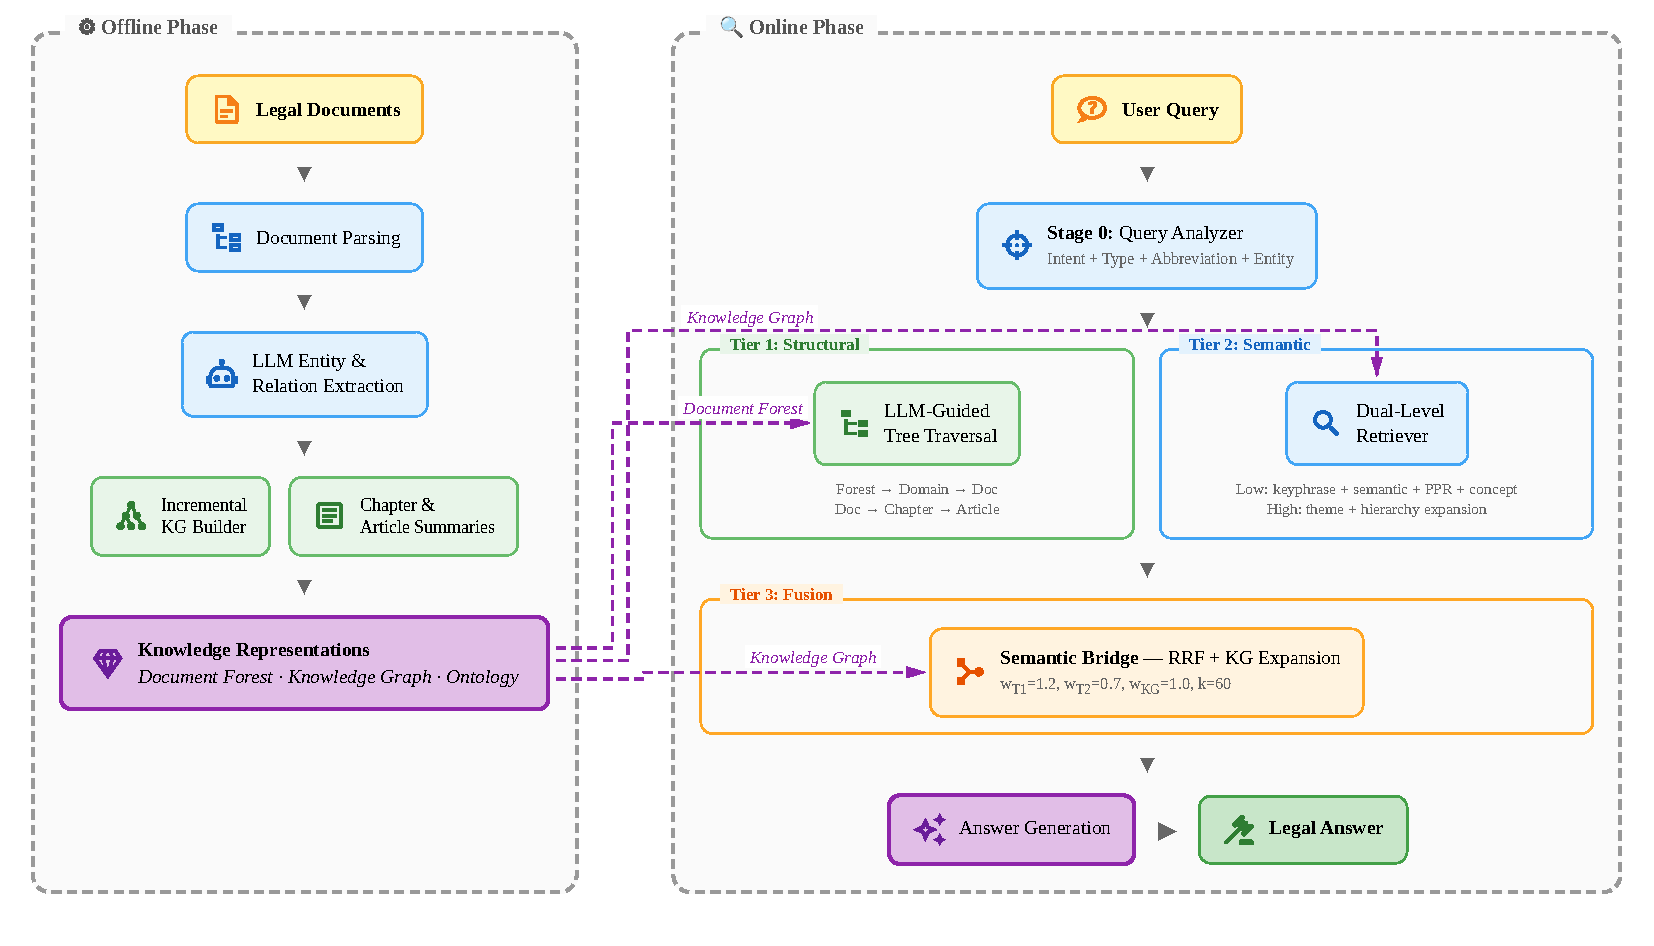
\includegraphics[width=\textwidth]{figure1-architecture.pdf}
\caption{Architecture of the proposed three-tier retrieval system. Offline phase (left): knowledge model construction from legal documents. Online phase (right): query processing through Tier~1 (structural tree traversal), Tier~2 (dual-level semantic retrieval), and Tier~3 (RRF fusion with KG expansion).}
\label{fig:architecture}
\end{figure}

\subsection{Knowledge Representation Model}

The model extends Legal-Onto \cite{r8}, which defines $K = (C, R, \textit{RULES}) + (\textit{Key}, \textit{Rel}, \textit{weight})$ integrating the Rela-model \cite{r21} with conceptual graphs. This extension separates terminological from assertional knowledge, adds structural representation, and replaces manual rules with LLM-based retrieval.

\begin{definition}[Legal Knowledge Model]
Given a legal corpus $\mathbf{D}$, the knowledge model is:
\begin{equation}
\mathbf{M} = (\mathbf{O}, \mathbf{G}, \mathbf{T}, \Phi)
\end{equation}
where $\mathbf{O}$ is a domain ontology, $\mathbf{G}$ is a knowledge graph, $\mathbf{T}$ is a document forest, and $\Phi$ is a set of retrieval functions.
\end{definition}

The ontology $\mathbf{O} = (C, P, H, L)$ represents terminological knowledge: OWL classes for legal entity types ($C$), object and datatype properties ($P$), a 4-level class hierarchy ($H$), and Vietnamese label mappings ($L$). This separates the TBox from Legal-Onto's flat concept set, enabling class hierarchy traversal for query expansion.

The knowledge graph $\mathbf{G} = (E, R)$ represents assertional knowledge: entities with 14 types (Table~\ref{tab:kg-stats}) and confidence scores, linked by 56 predicate types with evidence text. Selected predicates are declared symmetric or transitive to support inference during PPR traversal. The ontology answers ``\textit{what kind of entity?}'' via taxonomy traversal, while the knowledge graph answers ``\textit{what rules apply?}'' by linking entities to governing articles.

\begin{definition}[Document Forest]
The document forest $\mathbf{T} = \{T_1, \ldots, T_m\} \cup X$ represents structural knowledge. Each $T_i$ is a rooted tree with six levels (Document${}\to{}$\allowbreak Chapter${}\to{}$\allowbreak Section${}\to{}$\allowbreak Article${}\to{}$\allowbreak Clause${}\to{}$\allowbreak Point), and $X$ contains cross-reference edges between documents. The forest spans multiple legal domains, with documents organized into domain groups that enable domain-aware routing during retrieval.
\end{definition}

The retrieval functions $\Phi = \{\phi_0, \phi_1, \phi_2, \phi_3\}$ replace Legal-Onto's manual inference rules with LLM-based retrieval: $\phi_0\colon Q \to Q'$ (query analysis), $\phi_1\colon Q' \times \mathbf{T} \to 2^A$ (tree traversal), $\phi_2\colon Q' \times \mathbf{G} \to 2^A$ (semantic retrieval), and $\phi_3\colon 2^A \times 2^A \times \mathbf{G} \to A^*$ (RRF fusion). Each function is detailed in Section~\ref{sec:tiers}.

\subsection{Knowledge Graph Construction}

The offline phase builds the knowledge graph in four stages: (1)~document parsing into hierarchical trees forming the document forest; (2)~entity-relation extraction via one LLM call per article, producing evidence-grounded triples; (3)~incremental KG building with Vietnamese slug normalization and 4-pass deduplication across all documents; (4)~summary generation for Tier~1 traversal. Following knowledge engineering practice \cite{r9}, construction is semi-automatic: after LLM extraction, evaluation on a development set revealed missing cross-document references. A domain expert then added $\sim$130 relations (cross-document references and concept entities linking legal terms to governing articles). This evaluate-and-refine loop contributes to the accuracy reported in Section~\ref{sec:experiments}.

Each query intent amplifies its most relevant relation types during PPR traversal, assigning weight 1.0 to primary relations (e.g., \textit{defines\_as} for Definition, \textit{has\_penalty} for Penalty) and 0.5 to others, with near-synonym relations receiving intermediate weights.

\subsection{Three-Tier Retrieval}
\label{sec:tiers}

\subsubsection{Stage 0: Query Analysis}

The query analyzer performs: (1)~intent classification into six types (Penalty, Definition, Procedure, Requirement, Reference, General) via Vietnamese regex with LLM fallback; (2)~query type assignment among seven categories for downstream routing; (3)~abbreviation expansion (e.g., \textit{TNHH} $\to$ \textit{trach nhiem huu han}); and (4)~entity extraction of article references, law references, and legal keywords to seed retrieval.

\subsubsection{Tier 1: LLM-Guided Tree Traversal}

Tier~1 navigates the document forest using LLM reasoning in three loops. Loop~0 (Forest$\to$Domain$\to$Document) first matches the query to a domain group using pre-computed domain keywords, then selects the top~5 documents within the matched domain. Loop~1 (Document$\to$Chapter) selects the top~8 chapters using summaries and keywords. Loop~2 (Chapter$\to$Article) identifies the top~7 articles from article summaries. General Provisions chapters are automatically included. Each loop produces a reasoning path for interpretable retrieval.

\subsubsection{Tier 2: Dual-Level Semantic Retrieval}

Tier~2 performs hybrid semantic search over the knowledge graph with six scoring components at two levels. At the low level (entity-specific): keyphrase matching, query-entity cosine similarity, and intent-aware PPR. At the high level (conceptual): legal theme identification and concept hierarchy traversal, surfacing related articles even without direct entity matches. The combined score is:
\begin{equation}
S_{\text{T2}} = .05 S_{\text{kp}} + .20 S_{\text{con}} + .25 S_{\text{PPR}} + .20 S_{\text{sem}} + .15 S_{\text{thm}} + .15 S_{\text{hier}}
\end{equation}

The PPR component computes query-specific node importance on the knowledge graph:
\begin{equation}
\text{PPR}(v) = (1-\alpha) \sum_{u \in N(v)} \frac{w(u,v) \cdot \text{PPR}(u)}{d(u)} + \alpha \cdot p(v)
\end{equation}
where $\alpha=0.15$ is the teleport probability, $w(u,v)$ is the edge weight adjusted by query intent (Section~3.4), $d(u)$ is the weighted out-degree of $u$, and $p(v)$ is the personalization vector seeded from matched entities.

\subsubsection{Tier 3: Semantic Bridge (RRF Fusion)}

Tier~3 merges results from Tier~1 and Tier~2 using Reciprocal Rank Fusion \cite{r28}:
\begin{equation}
\text{RRF}(d) = \sum_{s \in \{T1, T2, KG\}} w_s \cdot \frac{1}{k + \text{rank}_s(d)}
\end{equation}
where $k=60$ and source weights are $w_{T1}=1.2$, $w_{T2}=0.7$, $w_{KG}=1.0$. Tree traversal receives the highest weight as it provides the most reliable structural signal; the gap between $w_{T1}$ and $w_{KG}$ allows dual-level retrieval and KG expansion to compensate when the LLM selects suboptimal chapters.

After initial fusion, results are expanded through the knowledge graph's relation edges. Strong relations (\textit{references}, \textit{requires}, \textit{depends\_on}) are expanded both cross-chapter (up to 5 articles) and same-chapter (up to 2 articles), with a semantic relevance filter (cosine similarity $\geq 0.4$) to suppress noise. After RRF scoring, $\pm 2$ adjacent articles from each result are added with decay factor 0.7, as correct answers often lie in neighboring articles. Top-ranked articles are then passed to an LLM for answer generation.

\section{Experiments}
\label{sec:experiments}

\subsection{Experimental Setup}

The evaluation corpus consists of 18 Vietnamese legal and regulatory documents spanning three domains. The enterprise law domain includes Law~59/2020/QH14 (Enterprise Law) and nine associated decrees, totaling 77~chapters and 840~articles. The traffic safety law domain covers Law~36/2024/QH15 and two penalty decrees. The education regulation domain comprises five postgraduate documents from UIT and VNUHCM, containing 109~articles. In total, the corpus contains 949~articles.

For evaluation, 530~questions were collected from LuatVietnam, ThuVienPhapLuat, and university portals, with expert annotations identifying 1--8 relevant articles per question (average~2.3). The questions are distributed across enterprise law (197), traffic safety law (203), and education regulation (130).

Table~\ref{tab:kg-stats} summarizes the constructed knowledge graph.

\begin{table}[H]
\centering\footnotesize
\caption{Knowledge graph statistics.}
\label{tab:kg-stats}
\begin{tabular}{lr@{\hskip 1.2cm}lr@{\hskip 1.2cm}lr}
\toprule
\textbf{Entity Type} & \textbf{Count} & \textbf{Relation Type} & \textbf{Count} & \textbf{Structure} & \textbf{Count} \\
\midrule
Total Entities & 5,936 & Total Relations & 5,963 & Tree Nodes & 9,226 \\
Action & 1,903 & requires & 1,377 & Documents & 13 \\
Legal Term & 1,632 & applies\_to & 810 & Chapters & 77 \\
Organization & 500 & has\_authority & 506 & Articles & 840 \\
Legal Reference & 451 & references & 434 & Cross-refs & 168 \\
Other (9 types) & 1,450 & Other (52 types) & 2,506 & & \\
\bottomrule
\end{tabular}
\end{table}

\textbf{Implementation.} The system is implemented in Python~3.11. Document parsing uses custom regex parsers for Vietnamese legal hierarchy detection. Entity extraction and knowledge graph construction employ Claude~3.5~Haiku\footnote{\url{https://www.anthropic.com/claude}} via the Anthropic API. Online query processing (tree traversal, query analysis) uses Claude Sonnet~4. Sentence embeddings are computed with paraphrase-multilingual-MiniLM-L12-v2\footnote{\url{https://huggingface.co/sentence-transformers/paraphrase-multilingual-MiniLM-L12-v2}}, a 384-dimensional multilingual model from the Sentence-Transformers library \cite{r2}. Vector similarity search uses FAISS\footnote{\url{https://github.com/facebookresearch/faiss}}, a library for efficient similarity search of dense vectors. Personalized PageRank is computed iteratively (max~50~iterations, tolerance~$10^{-6}$) using NumPy. All LLM responses are cached in SQLite for reproducibility.

\textbf{Metrics.} Since each query has expert-annotated relevant articles, we adopt standard retrieval metrics \cite{r19} that enable objective, reproducible evaluation against known ground truth, rather than LLM-as-judge scores used in open-ended generation benchmarks. Hit@$k = \frac{1}{|Q|}\sum_{q} \mathbf{1}[\exists\, a \in R_q : \text{rank}(a) \leq k]$ measures the fraction of queries for which at least one relevant article appears in the top-$k$ results, where $R_q$ denotes the set of relevant articles for query $q$. Mean Reciprocal Rank is defined as MRR $= \frac{1}{|Q|}\sum_q (\min_{a \in R_q} \text{rank}(a))^{-1}$, averaging the reciprocal rank of the first relevant result. Recall@$k$, Precision@$k$, and NDCG@$k$ \cite{r19} are also computed. Results are reported at $k \in \{1, 3, 5, 10, 20, 30\}$, with Hit@10 and MRR as the primary metrics. Hit@10 is prioritized because in a RAG pipeline the LLM provides an additional validation layer over retrieved context, at least one correct article among ten candidates suffices for accurate answer generation while limiting noise that could induce hallucination. MRR complements Hit@10 by rewarding higher placement of relevant articles, reducing irrelevant context that the LLM must filter.

\subsection{Baselines}

BM25 \cite{r18} ($k_1\!=\!1.2$, $b\!=\!0.75$); TF-IDF \cite{r19} with syllable-level tokenization and Vietnamese stopword removal; NaiveRAG \cite{r2} (dense retrieval with multilingual sentence-transformers, no reranking); LightRAG\footnote{\url{https://github.com/HKUDS/LightRAG}} \cite{r5} with Vietnamese entity extraction and default parameters, using the same LLM backend as the proposed system; RAPTOR\footnote{\url{https://github.com/parthsarthi03/raptor}} \cite{r29} with collapsed-tree retrieval using LLM-generated summaries (Sonnet~4 for summarization, MiniLM for embeddings); PageIndex\footnote{\url{https://github.com/pdfToTree/PageIndex}} \cite{r7} with two-step hierarchical tree search (document$\to$chapter selection, then chapter$\to$article selection), using heuristic summaries extracted from article text. All baselines use Sonnet~4 for online queries and retrieve from the full corpus with max\_results=30.

\subsection{Main Results}

The proposed system achieves 92.2\% Hit@10 (MRR 0.603), outperforming PageIndex by 7.4\% and the best traditional baseline (Keyword) by 43.7\% (Table~\ref{tab:main-results}). PageIndex (84.8\%) benefits from tree-based structural navigation but misses cross-reference articles outside the traversal path. Notably, RAG baselines (NaiveRAG 32.8\%, LightRAG 39.8\%, RAPTOR 41.0\%) underperform even BM25 (47.5\%). This is consistent with findings on domain-specific benchmarks \cite{r19}: general-purpose embeddings lack Vietnamese legal vocabulary, and generic KG extraction introduces noise rather than precision. RAPTOR's summaries further lose article-level granularity. BM25 succeeds through exact term matching but lacks structural awareness. The proposed system overcomes both limitations via LLM-guided navigation and domain-specific knowledge graph.

\begin{table}[H]
\centering\footnotesize
\caption{Legal domain Hit@$k$ (\%) on 400 questions. Best in bold, second \underline{underlined}.}
\label{tab:main-results}
\begin{tabular}{l@{\hskip 3pt}r@{\hskip 3pt}r@{\hskip 3pt}r@{\hskip 3pt}r@{\hskip 3pt}r}
\toprule
\textbf{Method} & \textbf{Hit@5} & \textbf{Hit@10} & \textbf{Hit@20} & \textbf{Hit@30} & \textbf{MRR} \\
\midrule
\multicolumn{6}{l}{\textit{Traditional retrieval}} \\
BM25 & 30.8 & 47.5 & 66.2 & 74.8 & 0.200 \\
TF-IDF & 29.2 & 45.8 & 64.5 & 74.8 & 0.207 \\
Keyword & 33.5 & 48.5 & 63.2 & 72.8 & 0.222 \\
\midrule
\multicolumn{6}{l}{\textit{RAG systems}} \\
NaiveRAG \cite{r2} & 22.8 & 32.8 & 51.8 & 60.5 & 0.146 \\
LightRAG \cite{r5} & 25.5 & 39.8 & 47.8 & 49.2 & 0.173 \\
RAPTOR \cite{r29} & 25.2 & 41.0 & 54.5 & 62.3 & 0.170 \\
PageIndex \cite{r7} & \underline{76.2} & \underline{84.8} & \underline{90.2} & \underline{91.0} & \underline{0.559} \\
\midrule
3-Tier (ours) & \textbf{74.5} & \textbf{92.2} & \textbf{94.8} & \textbf{95.0} & \textbf{0.603} \\
\bottomrule
\end{tabular}
\end{table}

\subsection{Multi-Domain Performance}

Table~\ref{tab:domain-results} reports per-domain results, including education as a generalization test.

\begin{table}[H]
\centering\footnotesize
\caption{Per-domain Hit@10 (\%) across three domains.}
\label{tab:domain-results}
\begin{tabular}{l@{\hskip 4pt}r@{\hskip 4pt}r@{\hskip 4pt}r}
\toprule
\textbf{Method} & \textbf{Enterprise (197)} & \textbf{Traffic (203)} & \textbf{Education (130)} \\
\midrule
NaiveRAG & 29.9 & 35.5 & 50.0 \\
LightRAG & 20.3 & 58.6 & 53.1 \\
RAPTOR & 18.5 & 63.5 & 53.8 \\
BM25 & 31.5 & 63.1 & 70.0 \\
TF-IDF & 39.1 & 52.2 & 68.5 \\
Keyword & 20.3 & 75.9 & 56.2 \\
PageIndex & \underline{76.6} & \underline{92.6} & \underline{74.6} \\
3-Tier (ours) & \textbf{86.5} & \textbf{98.0} & \textbf{88.5} \\
\midrule
\textit{Ours vs.\ PageIndex} & \textit{+9.9} & \textit{+5.4} & \textit{+13.9} \\
\bottomrule
\end{tabular}
\end{table}

The system outperforms all baselines across all three domains. Traffic law achieves the highest Hit@10 (98.0\%) due to direct violation-to-penalty mappings. Enterprise law is harder (86.5\%) due to cross-decree references. Education regulation (88.5\%) demonstrates generalization: the largest margin over PageIndex (+13.9\%) occurs here, where semantic retrieval captures terminology that tree navigation misses. No domain-specific tuning was applied.

\subsection{Analysis}

On the legal domain, Hit@10 ranges from 0\% (household business, 4~queries referencing articles outside the corpus) to 100\% (speed-related penalties), with most categories above 85\%. Company establishment (68.4\%) remains challenging due to cross-decree dependencies.

A multi-hop example illustrates tier cooperation: ``If a member borrows money to meet charter capital and later withdraws it, what are the penalties?'' requires linking concepts across chapters. Tier~1 reaches Art.\,47 (member obligations) via tree traversal; PPR walks \textit{requires} edges from ``charter capital'' to Art.\,16\,Cl.\,5 (prohibited acts) in a different chapter; RRF places both in the top~5. No baseline answers this query at Hit@30.

Of the 31 missed queries (7.8\%), 27 involve enterprise law. Primary failure modes: company establishment across multiple decrees (6~queries), household business outside the corpus (4~queries), and multi-article queries ($>$2 expected) accounting for 14 of 31 misses.

\section{Conclusion}
\label{sec:conclusion}

This paper presented a three-tier knowledge graph RAG architecture for Vietnamese legal question answering. The central contribution is a unified retrieval pipeline combining structural tree traversal, semantic graph search with intent-aware Personalized PageRank, and Reciprocal Rank Fusion, grounded in a formal knowledge model extending the Legal-Onto framework. Experiments across three domains demonstrate consistent superiority over all baselines without domain-specific tuning.

Limitations include Tier~1 latency (approximately 7 seconds per query due to multiple LLM calls); however, in the legal domain, retrieval accuracy takes priority over response speed. A remaining limitation is lower performance on enterprise law queries requiring multi-document cross-references. Future work includes extension to additional regulatory domains, multi-turn conversational support, and explainable retrieval traces.

\section*{Acknowledgments}
This research is funded by University of Information Technology, Vietnam National University Ho Chi Minh City, Vietnam.

\bibliographystyle{unsrt}
\bibliography{references}

\end{document}
